
% ==================================================================
\section{GENFORM} \label{genform}


% -----------------------------------------------------------------
\subsection{What is GENFORM?}

GENFORM means “generic form” and is a WebObs integrated tool to create a \wo{form} with user-defined database fields, configurable form layout and display/export table of selected data. The form can be associated to a \wo{proc} which define the associated \wo{nodes}. Each record is associated to a single \wo{node} of the \wo{proc}. Data associated to a GENFORM can be read by the proc without the need of defining RAWFORMAT and RAWDATA.

When creating a new \wo{form}, you can define it from a selection of various templates, and modify it as you wish. Once created, a \wo{form} can be modified by adding new inputs and/or change the form layout, but previous inputs cannot be deleted: if an input is not used anymore, it can be ignored and simply remove from the form layout fields.

A GENFORM is defined by its configuration file (based on the \wokey{key|value} model) with a specific syntax defining the input fields (name, unit and type) and form layout.


% - - - - - - - - - - - - - - - - - - - - - - - - - - - - - - - - -
\subsubsection{Data structure}

Each \wo{form} is then associated to a table in a database called \wofile{WEBOBSFORMS.db}. Each table of the database use the scheme shown in table \ref{table:genform_db}.

\begin{table}[h]
	\centering
	\begin{tabular}{c c l}
		\hline
		\textit{Name} & \textit{Type} & \textit{Comment} \\
		\hline
		{\tt id}         & integer  & primary key autoincrement\\
		{\tt trash}      & boolean  & True = bin	\\
		{\tt quality}    & integer  & 0 = raw, 1 = validated \\
		{\tt node}       & text     & WebObs ID of the associated \wo{node} \\
		{\tt edate}      & datetime & date and time end of measurement/collect/sampling \\
		{\tt edate\_min} & datetime & uncertainty date and time end of measurement \\
		{\tt sdate}      & datetime & date and time of optional start of measurement \\
		{\tt sdate\_min} & datetime & uncertainty date and time start of measurement \\
		{\tt users}      & text     & WebObs UID or GID of the operators (authorized list) \\
		{\tt comment}    & text     & \\
		{\tt tsupd}      & timestamp & last edit timestamp \\
		{\tt userupd}    & text     & last edit user UID \\
		{\tt input01}    & text     & data n°1 \\
		{\tt input02}    & text     & data n°2 \\
		...              & text     & data n°... \\
		\hline
	\end{tabular}
	\caption{Scheme of the GENFORM database (each table).}
	\label{table:genform_db}
\end{table}

Each data record in a \wo{form} uses this structure:
\begin{itemize}
	\item an automatic unique identifier (for the database);
	\item a trash flag for deleted record;
	\item a quality number;
	\item an associated \wo{node};
	\item a start date/time and a end date/time: the start date/time is optional and may be automatically filled by the end date/time value if only one date is used in the \wo{form}. To manage date/time uncertainty, each date/time is associated to a companion minimum date/time to define an interval. For example, if the time of a record is unknown, the main date/time will contain yyyy-mm-dd 23:59:59 and the min date/time will contain 00:00:00 so that the full day is covered. This behavior is transparent for the user who have the possibility to set some fields empty (month, day, hour, and minute);
	\item a list of users/operators associated to the record. Users must be defined in the \wo{users} \webobs database;
	\item a comment field (text string);
	\item an automatic timestamp (last edit);
	\item the user who made the last edit (automatic);
	\item and the list of input field.
\end{itemize}

% -----------------------------------------------------------------
\subsection{Creation of a FORM} \label{genform_creation}

To create a new \wo{form} using GENFORM, you have to go in the \wo{grid} menu list and click on the pencil next to \textbf{Raw Data}. Then, you have to choose a name for the FORM and select a template that will be used to help you through the creation process. Currently, 3 templates exist:

\begin{itemize}
	\item GENFORM: the most basic template that shows you all the different types of inputs that you can use in GENFORM
	\item WATERS: a template based on the former EAUX \wo{form} used for the water chemistry analysis
	\item VOLCGAS: a template based on the former GAZ \wo{form} used for the gas chemistry analysis
	\item EXTENSO: a template based on the former EXTENSO \wo{form} used for the extensometer measurements
\end{itemize}

\begin{figure}[!h]
	\centering
	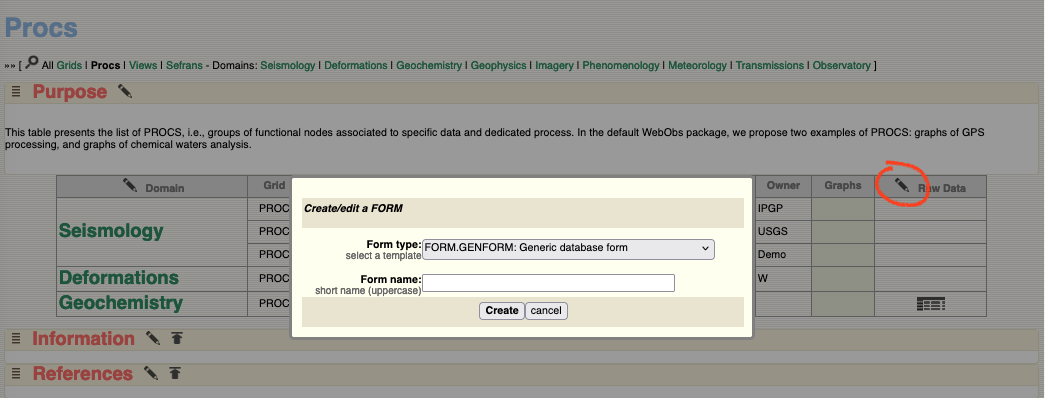
\includegraphics[width=\textwidth]{figures/GENFORM_creation.png}
	\caption{To create a form, click on the edit pencil, choose a template in the list and enter a short name.}
	\label{GENFORM_creation}
\end{figure}

If you want to edit a \wo{form}, you just need to go in the GENFORM creation menu and write the name of the \wo{form} you want to edit, no matter the template which is selected (see figure \ref{GENFORM_creation}).


% -----------------------------------------------------------------
\subsection{General parameters}


A GENFORM \wo{form} has general parameters:
\begin{itemize}
	\item a \wokey{TITLE} (long string) displayed on the pages referring to the \wo{form},
	\item a \wokey{BANG}, which is the oldest year of potential record in the \wo{form},
	\item a \wokey{STARTING\_DATE} flag which is a boolean, allowing GENFORM to define a starting date of each record in addition to end date,
	\item an \wokey{OPERATORS\_LIST}, list of operators as user UIDs and/or group +GIDs,
	\item the number of \wokey{COLUMNS} separating the form layout,
	\item the number of \wokey{FIELDSETS} used to group fields (inputs and outputs, see below) into categories.
\end{itemize}

% -----------------------------------------------------------------
\subsection{Fieldsets}

Each FIELDSET is referenced with a 2-digit number {\it xx}, has a name, a number of CELLS dividing it, and the list of the fields (INPUT or OUTPUT) you want to display in each CELL. CELLS are arranged into columns (the default), or into rows inside the FIELDSET. Finally, each CELL has a list of the fields you want to display in: \wokey{INPUTzz} and/or outputs \wokey{OUTPUTzz}. Fields are arranged vertically in the CELL if the FIELDSET is splitter into columns, or horizontally if splitted into rows.

FIELDSET parameters are for the fieldset {\it xx}:
\begin{itemize}
	\item \wokey{FIELDSETxx\_NAME}: full name of the fieldset, used in the form layout and table column header,
	\item \wokey{FIELDSETxx\_CELLS}: the number of cells inside the fieldset, followed by optional tag COLS (default) or ROWS,
	\item \wokey{FIELDSETxx\_Cyy}: list of INPUT and/or OUTPUT to display into the CELL {\it yy},
	\item \wokey{FIELDSETxx\_TOGGLE}: if YES, indicates that the fieldset will not be displayed by default in the table.
\end{itemize}

% -----------------------------------------------------------------
\subsection{Inputs and outputs fields}

The FIELDS in a GENFORM can be INPUTS, referencing to data that will be recorded into the database, and OUTPUTS, text or products to be displayed, like formulas, but not recorded.

INPUTS and OUTPUTS are referenced with a 2-digit number {\it zz}, have a name (mandatory), a unit, and a type. Common parameters are defined as suffix of \wokey{INPUTzz} or \wokey{OUTPUTzz}:
\begin{itemize}
	\item \wokey{\_NAME}: name of the field, preferably short since it is used in the table headers,
	\item \wokey{\_UNIT}: unit of the field (if relevant), indicated into parenthesis,
	\item \wokey{\_TYPE}: type of the field (see below),
	\item \wokey{\_FILT}: for list only, if \wokey{YES}, the list will be used as a filter in the table show,
	\item \wokey{\_VALID}: 2 threshold values in a list {\it a, b} (see below),
	\item \wokey{\_HELP}: a string to be displayed as window popup to explain the field containt.
\end{itemize}

% - - - - - - - - - - - - - - - - - - - - - - - - - - - - - - - - -
\subsubsection{Input types}

Valid TYPE for an INPUT field is:
\begin{itemize}
	\item \wokey{numeric(size):~\textit{default value}}: numeric input, optional size in characters (default is 5), and optional default value. This is the default input type if not specified;
	\item \wokey{text(size):~\textit{default value}} : text string, optional size in characters (default is 5), then optional default value;
	\item \wokey{list:~\textit{filename}}: name of a config file containing a \wokey{key|value} list of selectable items. It is also possible to use a \wokey{key|name|icon} 3-column config file, so that small icons will be displayed in table (instead of key), and radio button will replace the selectable list. If not exist, the file will be created after the first form save, from a template, and an edit link will be available;
	\item \wokey{users(size): \textit{list of UID and/or +GID}}: a list of users or group of users. Size stands for the menu length (default is 1);
	\item \wokey{image(size)}: file name of an image, with optional height size (in pixel, default is 50 px) for thumbnail display;
	\item \wokey{checkbox:~\textit{checked}}: boolean value as check box, optional default checked.
\end{itemize}

% - - - - - - - - - - - - - - - - - - - - - - - - - - - - - - - - -
\subsubsection{Output types}

Valid TYPE for an OUTPUT field is:
\begin{itemize}
	\item \wokey{formula(size):~\textit{formula}}, which allows to make simple mathematical operations between the different inputs and/or outputs (see below). Optional size of the result in characters (default is 6), and (size-3) significant digits; set the size to \wokey{0} to hide the formula (see below).
	\item \wokey{text} : text string (HTML allowed).
\end{itemize}

% - - - - - - - - - - - - - - - - - - - - - - - - - - - - - - - - -
\subsubsection{Formulas}

In formulas, the use of previous outputs is allowed but they must precede the current formula (with lower output numbers). The syntax must remain simple since the same formula is interpreted by Javascript in the form page and by Perl in the table page. Use of plus (+), minus (-), divide (/), multiply (*), exponent (**) operators, numbers and parenthesis is admitted, also some basic functions like \wokey{sqrt()}, \wokey{log()}, etc. An input must be referenced as \wokey{INPUTzz}, an output as \wokey{OUTPUTzz}, uppercase. It is possible to define hidden formula by setting the size to zero (0), but the field still MUST be included in a fieldset cell in order to be computed properly; this can be useful to calculate intermediate results used in other formula and not display it.
 
% - - - - - - - - - - - - - - - - - - - - - - - - - - - - - - - - -
\subsubsection{Color background threshold}

The VALID parameters applies to input or output of numeric/formula types. It contains a coma-separated list of 2 threshold values {\it a, b} to display color background associated to a level of validity of the field absolute value. Three levels of validity are defined: normal (green), warning (orange), and error (red). The criteria are, where {\it x} is the field value:
\begin{itemize}
	\item normal for abs({\it x}) $<=$ {\it a},
	\item warning for {\it a} $<$ abs({\it x}) $<=$ {\it b},
	\item error for abs({\it x}) $>$ {\it b}.
\end{itemize}

The 3 validity level colors can be defined in \wokey{VALIDITY\_COLORS} variable, for normal, warning, and error levels, respectively. Note that normal level color applies only in the form; for table display of data the normal level value has no background color (for readability).



% -----------------------------------------------------------------

\begin{table}[htp]
\caption{GENFORM template}
\label{genform_template}
\lstinputlisting{../../CODE/tplates/FORM.GENFORM}
\end{table}


